\subsection{Domænemodel}

Med en objektmodel opstillet kan vi gå videre og oprette en domænemodel.
Hvert domæne repræsentere et eller flere objekter i figur \ref{fig:Objektmodel}.    
Domænemodellen har sammen med objektmodellen også gennemgået flere iterationer, hvor domænerne er blevet uddybbet og nogen af dem fjernet.

\begin{figure}[H]
    \makebox[\textwidth][c]{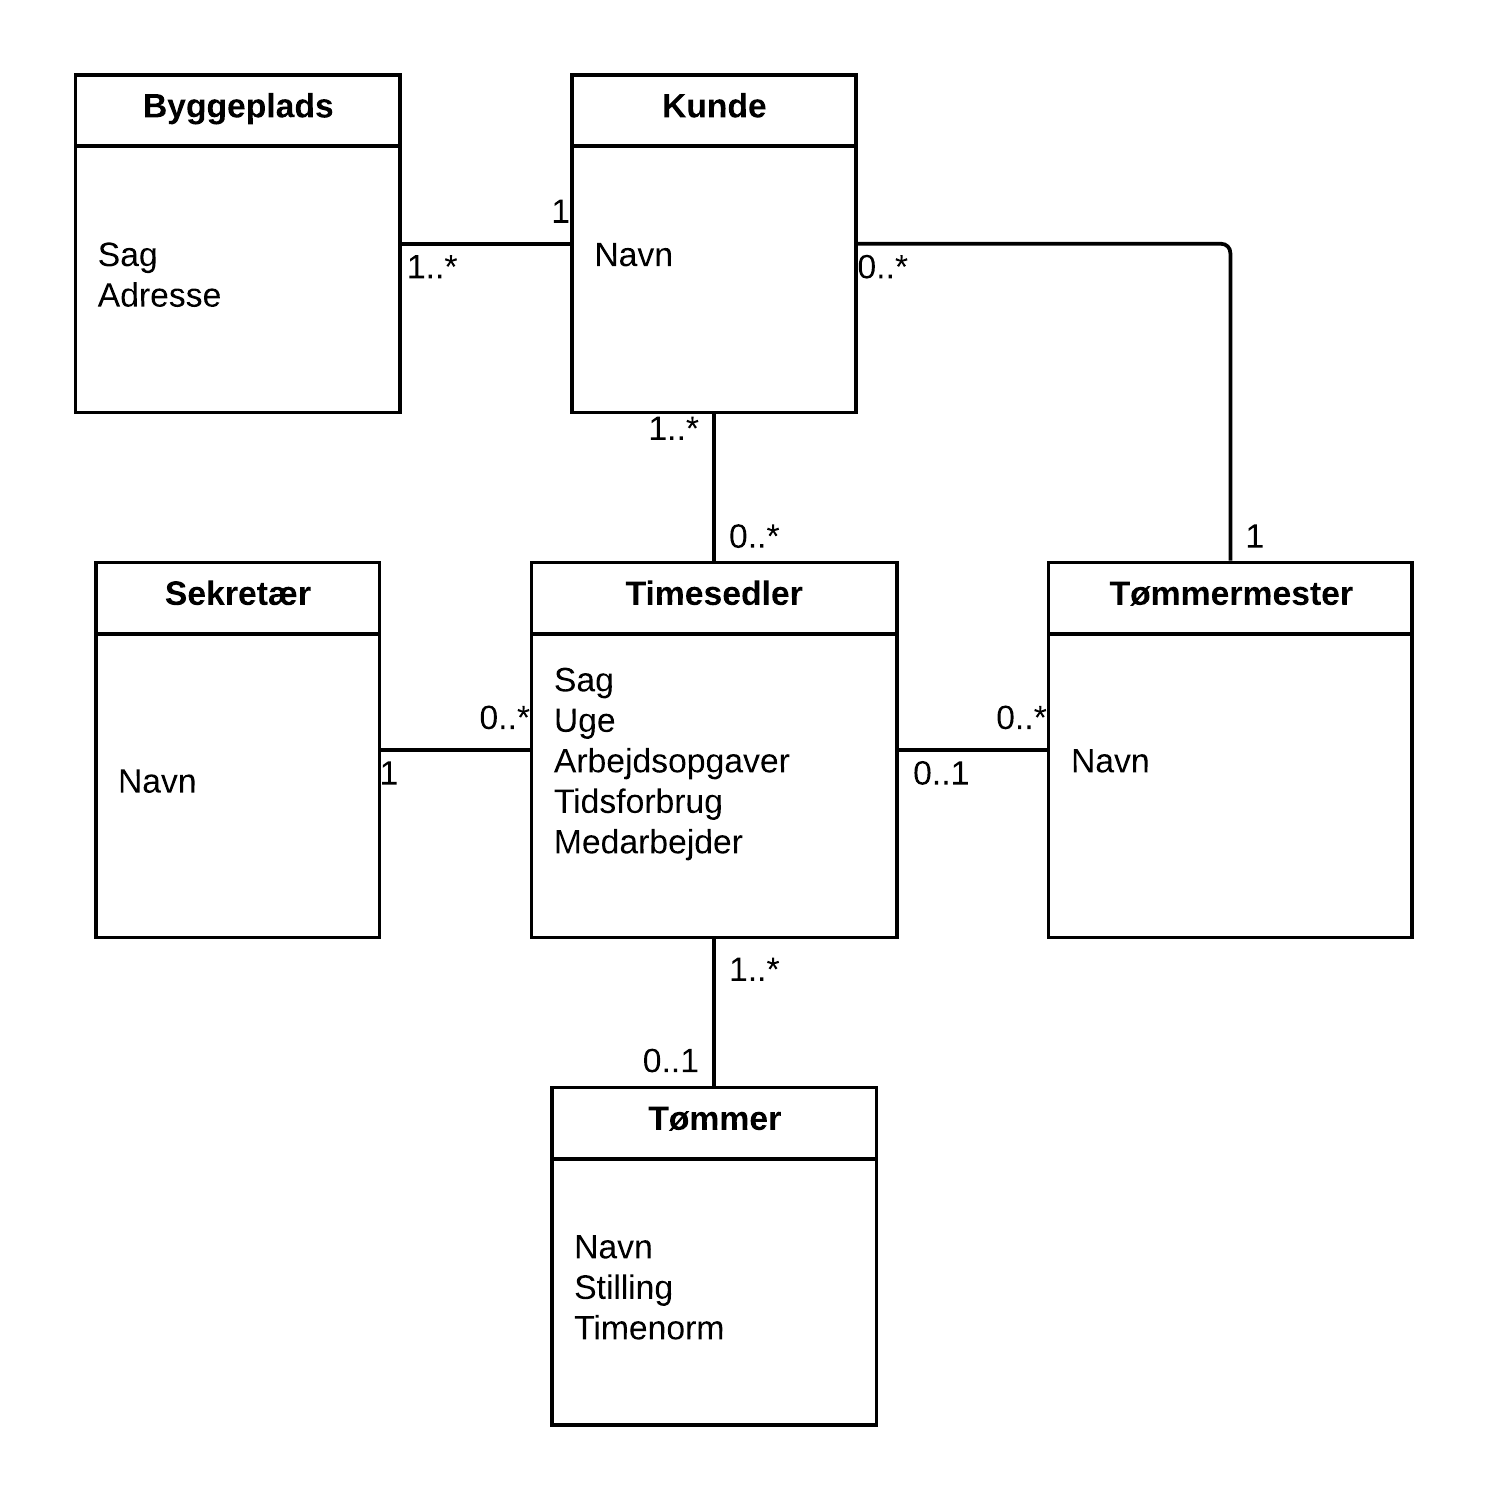
\includegraphics[scale = .6]{DomaenemodelSprint2.png}}
    \caption{Domænemodel: Her ses de domæner, der er relevante i forbindelse med tidsregistrering.}
    \label{fig:DomaeneModelSprint2}
\end{figure} 

Med hensyn til forholdene mellem domænerne har timeseddel domænet mange relationer til andre domæner, da timesedlen skal bruges både af sekretæren og tømmerne, mens den samtidig skal indeholde information omkring tømrerne.

Domænemodellen har taget udgangspunkt i at skabe et program for at gøre timeregistrering nemmere. Ud fra vejledningen og erfaringen fra objektmodellen afskaffede vi også værksteds og leverandørs. Ved evt. videreudvikling kunne det være relevant at indfører sådanne klasser, men eftersom de to klasser ikke havde nogen relevans til vores prioriteret PBI blev de undladt. Se afsnit \ref{vidud} for mere.